%!TEX root = Memoria_TFM.tex
\section{Databases}
Some databases has been used in order to learn, compare results and carry out the project. All the databases are formed by three subsets whose samples are not repeated among subsets: train, validation and test.

\begin{itemize}
\item The training subset is used to train the network during epochs. To know how the training behavior, a cost is calculated.
\item The validation subset is used to check the behavior of the network while is training, also, the validation subset is usually used to calculate the hyper-parameters of the network, although the hyper-parameters are not calculated until is pointed. The validation error is calculated for each training epoch. The metric use to the validation is $error(\%) = cost*100$.
\item  The test subset, that is used just at the end of the training. The best model is chosen with regard to the best validation error. Different metrics are going to be used for after testing the network (error rate(\%), TP, FP ...).
\end{itemize}

\subsection{MNIST digit database}\label{subsec:MNIST}
MNIST digit database is a image database of human written digits. This database is commonly used to learn machine learning techniques. Because of that, this database has been used, in this thesis, for learning Theano and convolutional neural networks. In addition, this database has been used in a implemented convolutional neural network (LeNet).\\
\begin{figure}[htb]
\centering
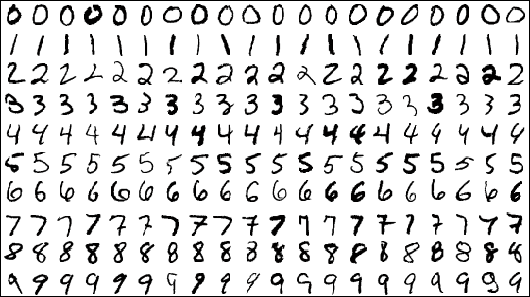
\includegraphics[width=0.6\textwidth]{images_databases/mnistExamples.png}
\caption{MNIST digit images database. Image obtained from \cite{MNISTimage}} \label{fig:MNIST_digits}
\end{figure}
Some examples of the digit image MNIST database could be seen in \ref{fig:MNIST_digits}, image obtained from \cite{MNISTimage} and the characteristics of this database are the following ones:

\begin{itemize}
 \item There are 70.000 number of unique samples.
 \item Altough original size of the database is 32x32 pixels, the samples of this downloaded database are 28x28 pixels in gray scale, that is 784 features per image.
 \item 10 classes could be differentiated, one per digit.
\item The samples are directly separated into train, test and validate subset.
\end{itemize}

\subsection{FRAV dataset}
FRAV database is an anti-spoofing face database built in the FRAV research group of tu URJC University and which is part of the Automated Border Control Gates for Europe project \cite{ABC4EU}.\\

One example of RGB images of FRAV database are shown in figure \ref{fig:RGB-frav1} and another example could be seen in \ref{fig:RGB-frav2}. In both images, the four attacks described previously and the real user could be visualized. \\

\begin{figure}[htb]
\centering
\subfigure[printed image attack]{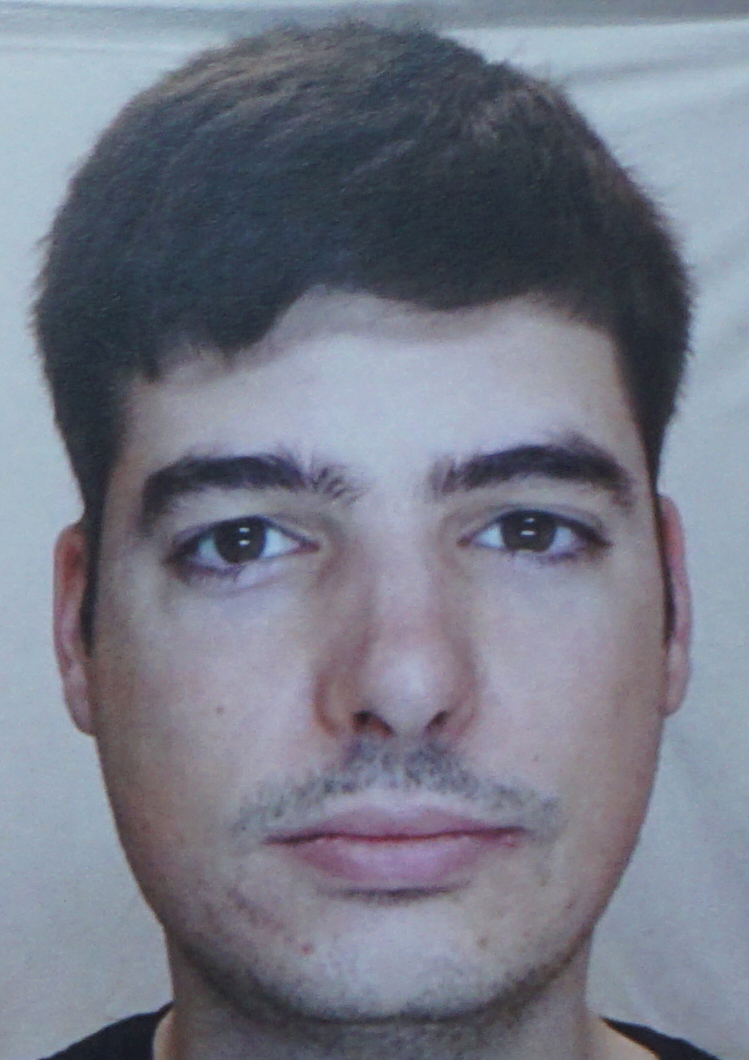
\includegraphics[width=0.18\textwidth]{images_databases/fravrgb/at1-0.JPG} \label{frav_im1-1} }
\subfigure[mask attack]{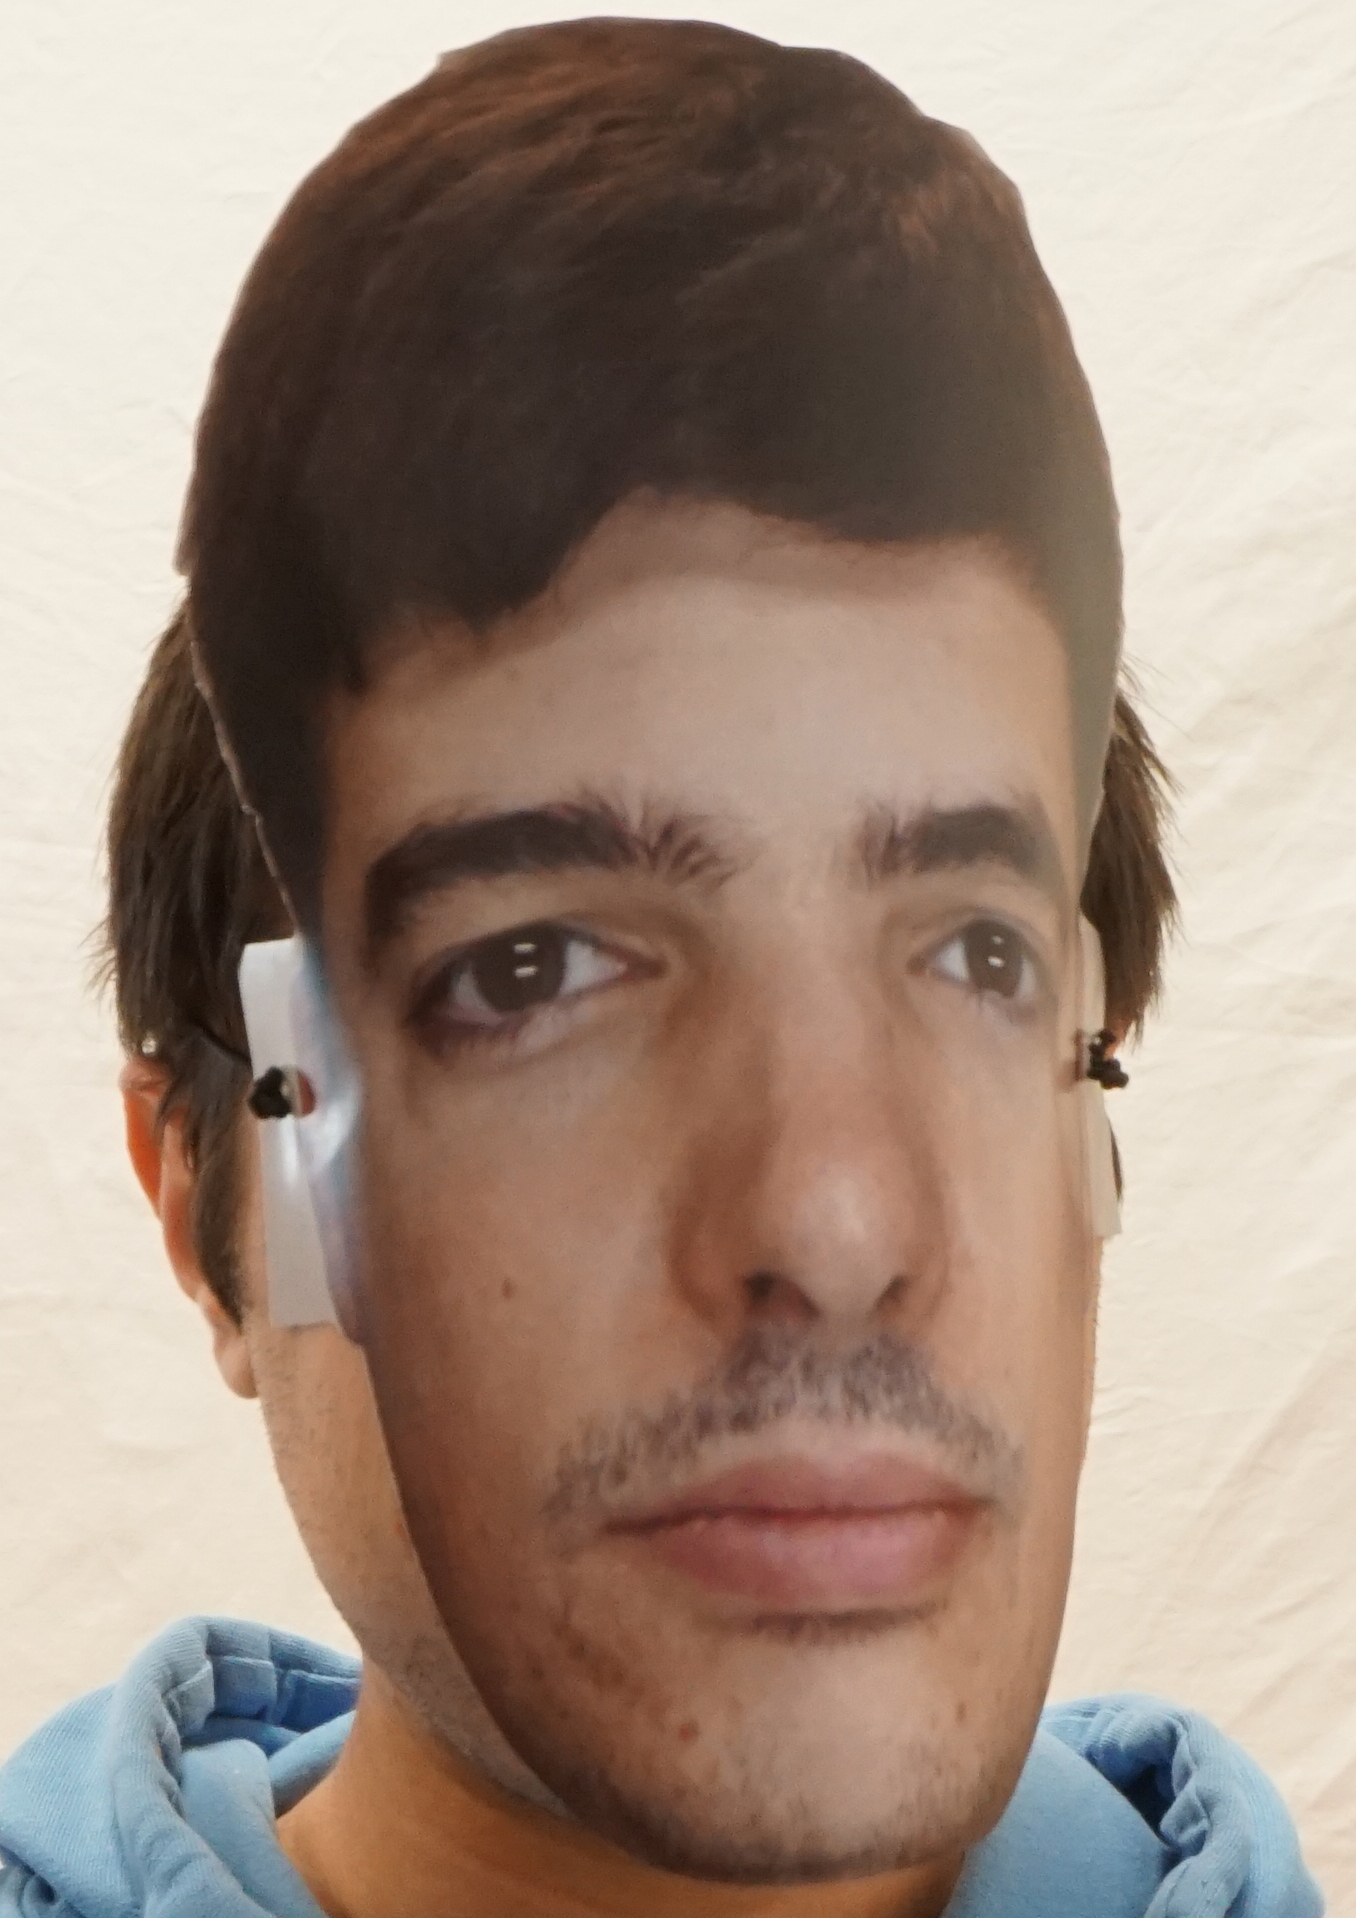
\includegraphics[width=0.18\textwidth]{images_databases/fravrgb/at2-0.JPG} \label{frav_im1-2}}
\subfigure[eye mask attack]{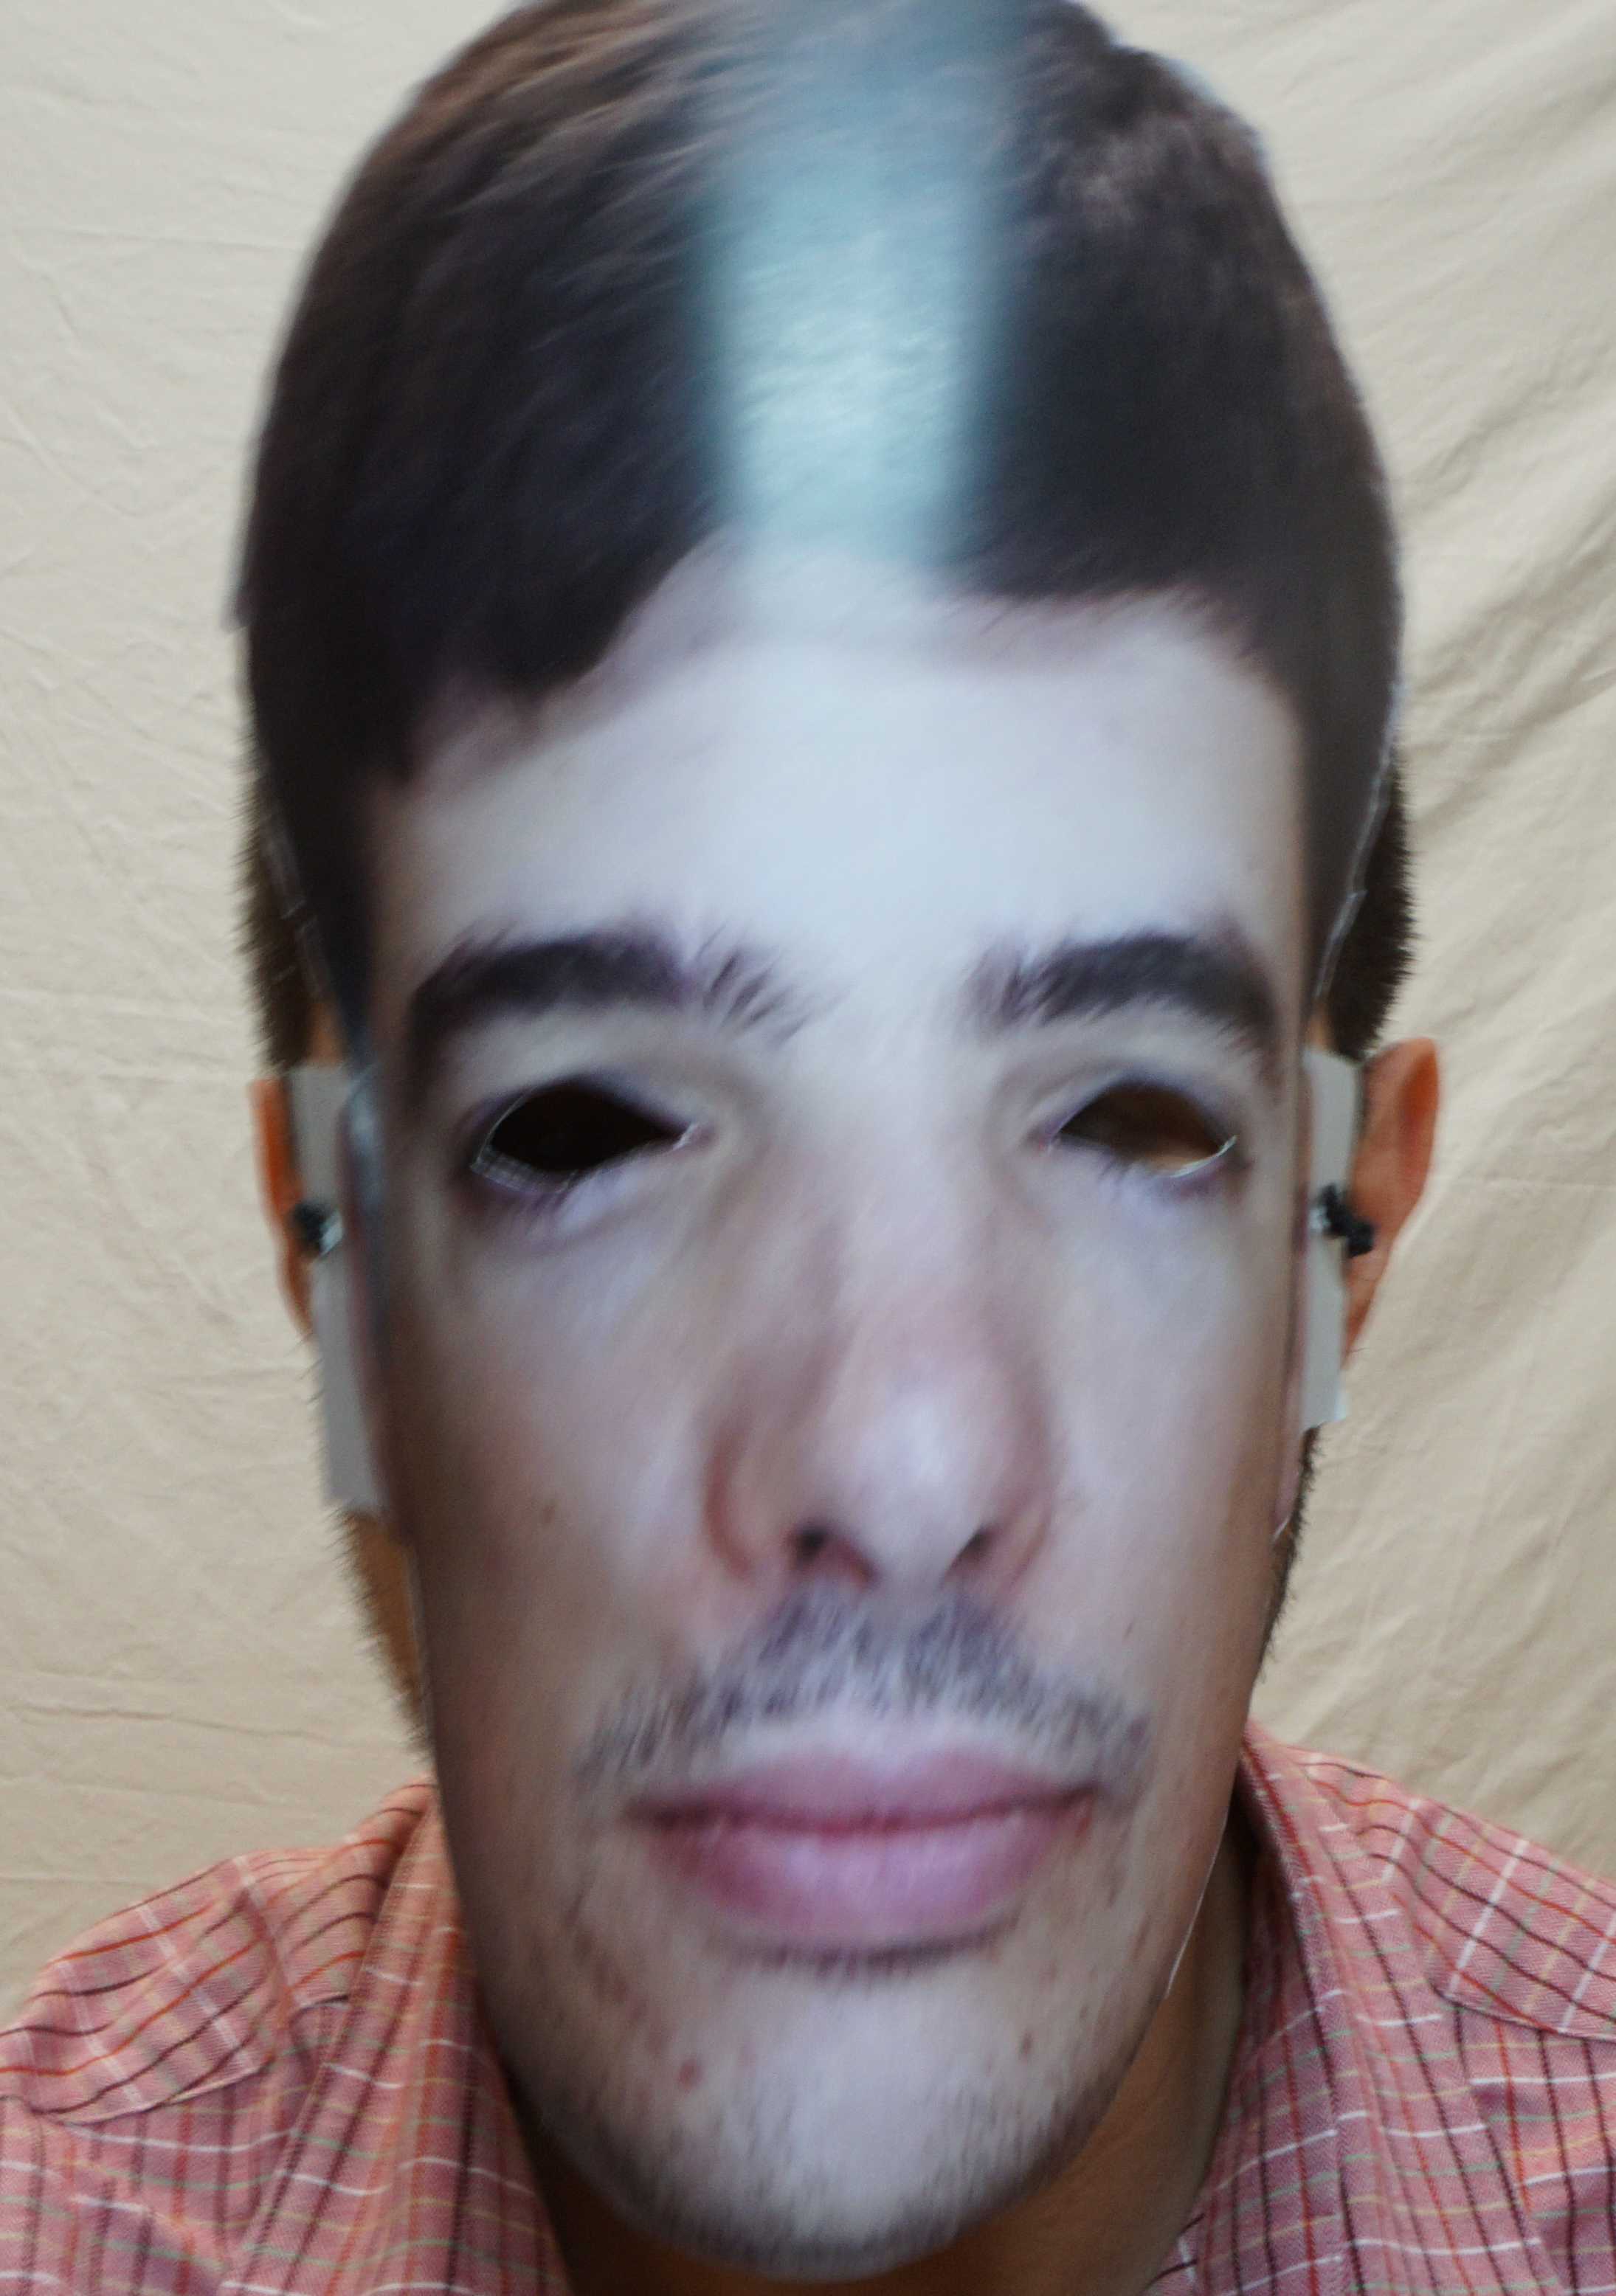
\includegraphics[width=0.18\textwidth]{images_databases/fravrgb/at3-0.JPG} \label{frav_im1-3}}
\subfigure[tablet attack]{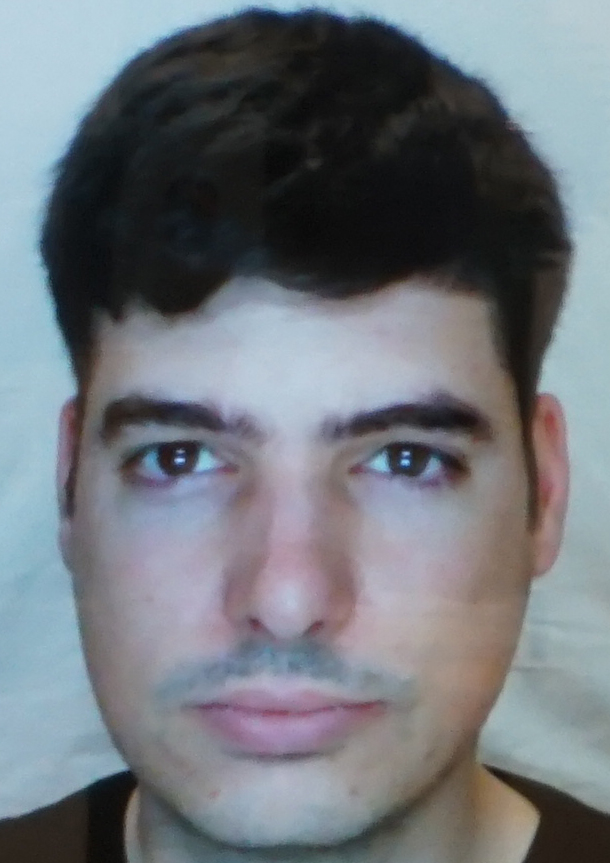
\includegraphics[width=0.18\textwidth]{images_databases/fravrgb/at4-0.JPG} \label{frav_im1-4}}
\subfigure[real user]{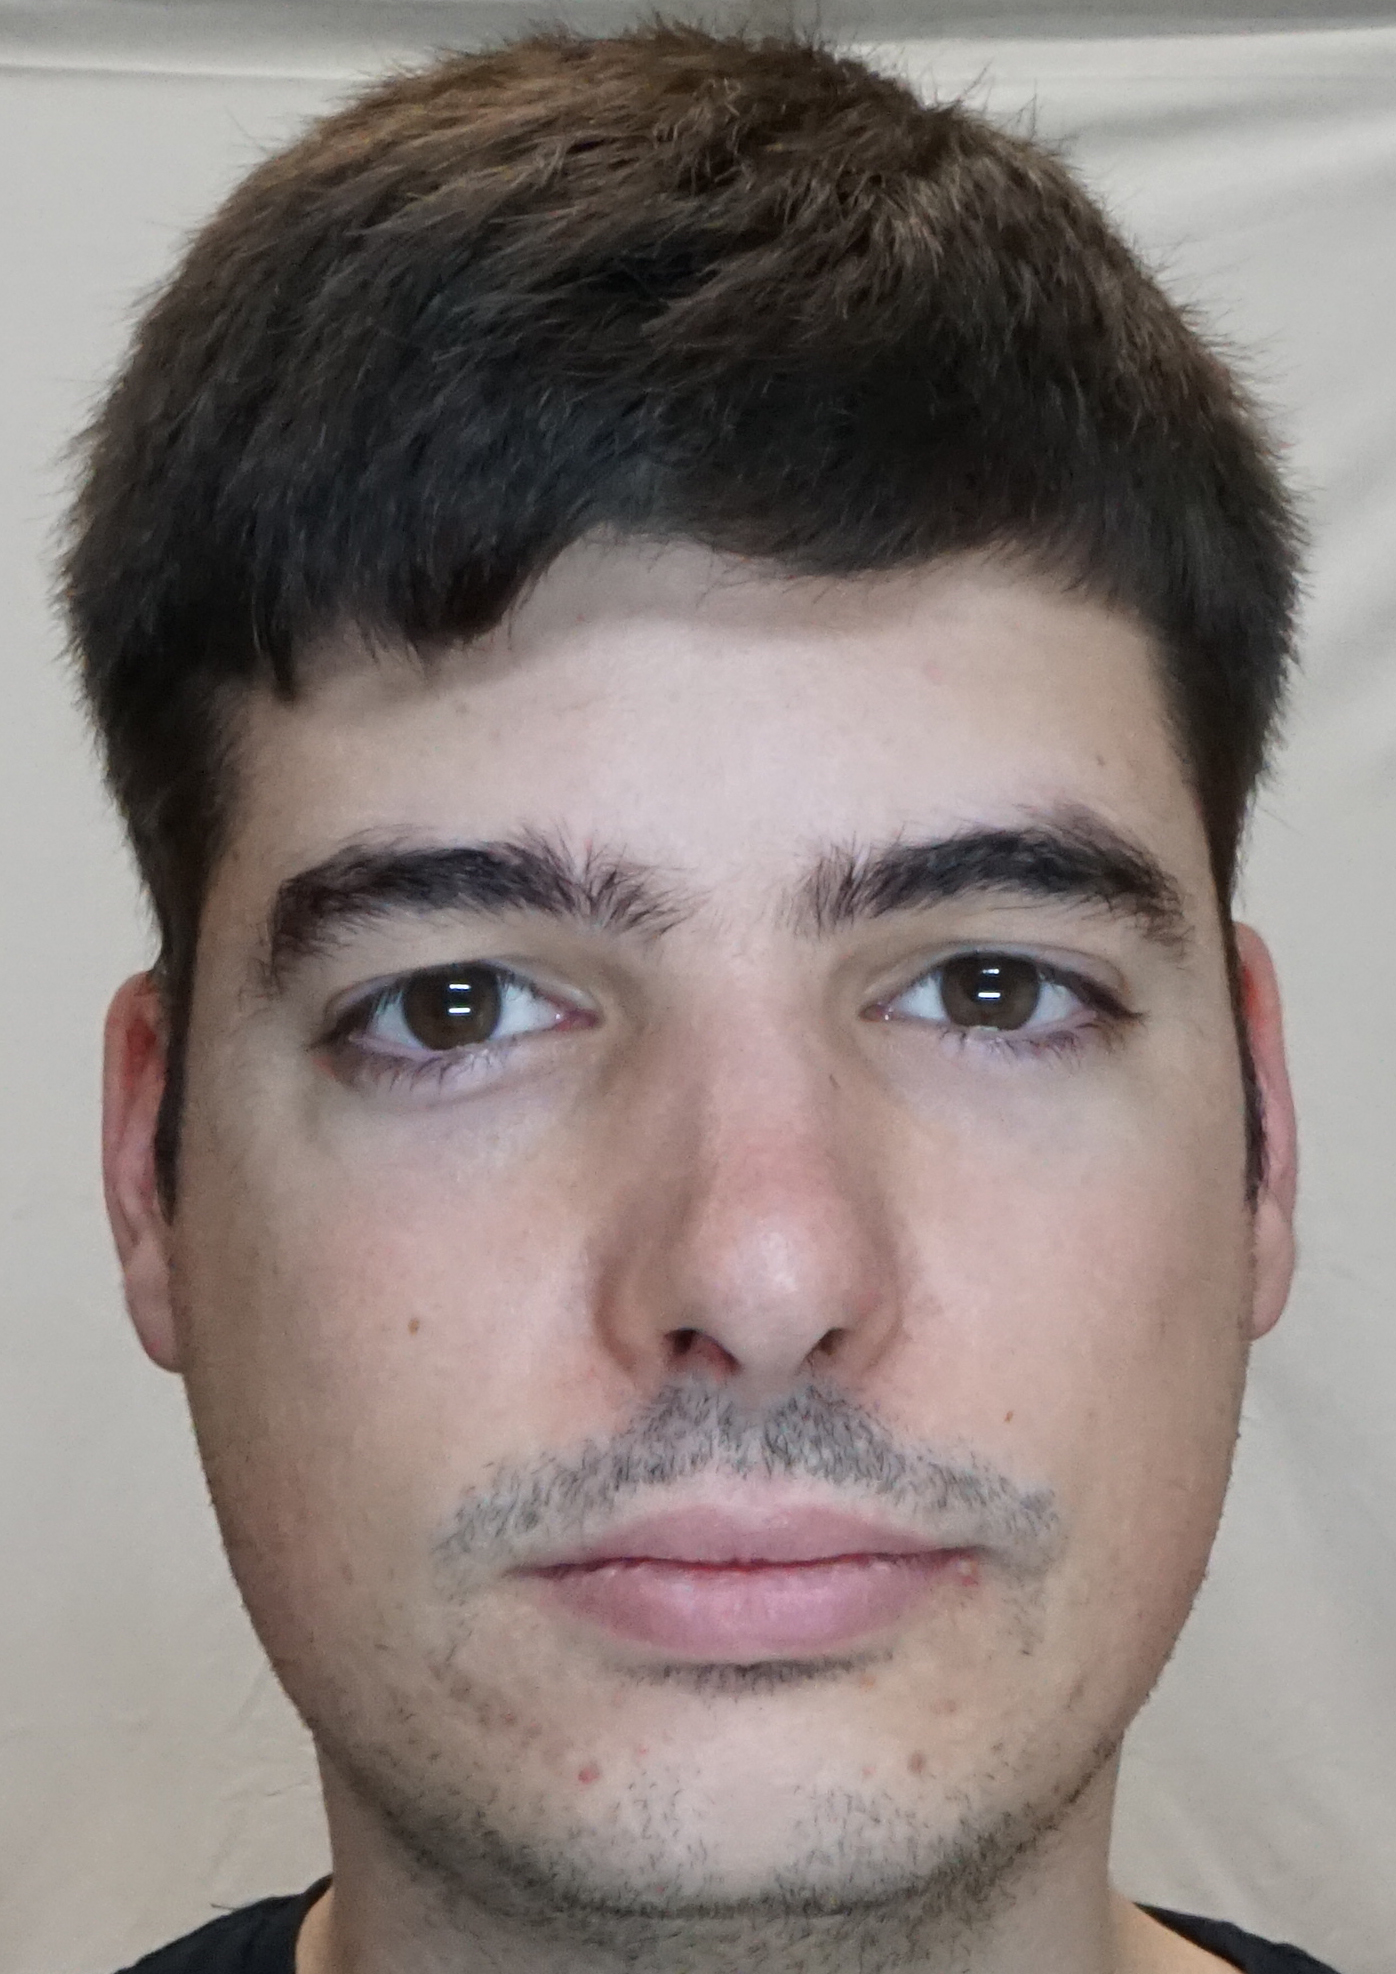
\includegraphics[width=0.18\textwidth]{images_databases/fravrgb/real0.JPG} \label{frav_im1-5}}

\caption{Four attacks and real user from RGB FRAV database } \label{fig:RGB-frav1}
\end{figure}

\begin{figure}[htb]
\centering
\subfigure[printed RGB image attack]{ 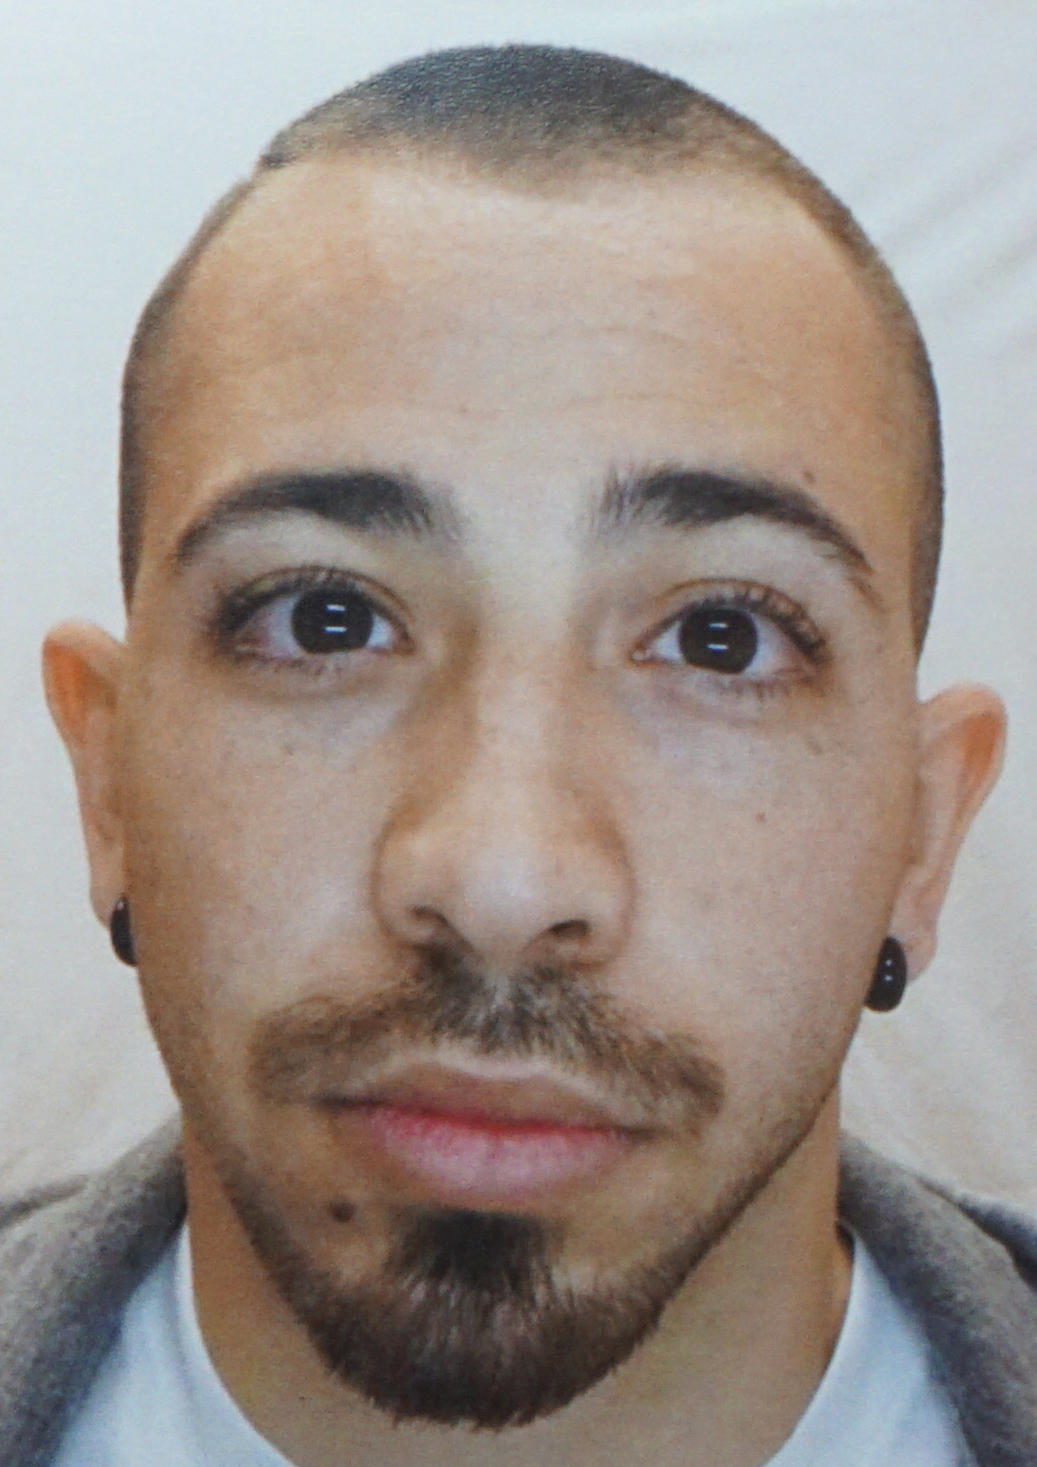
\includegraphics[width=0.18\textwidth]{images_databases/fravrgb/at1-1.JPG} \label{frav_im2-1} }
\subfigure[mask attack RGB]{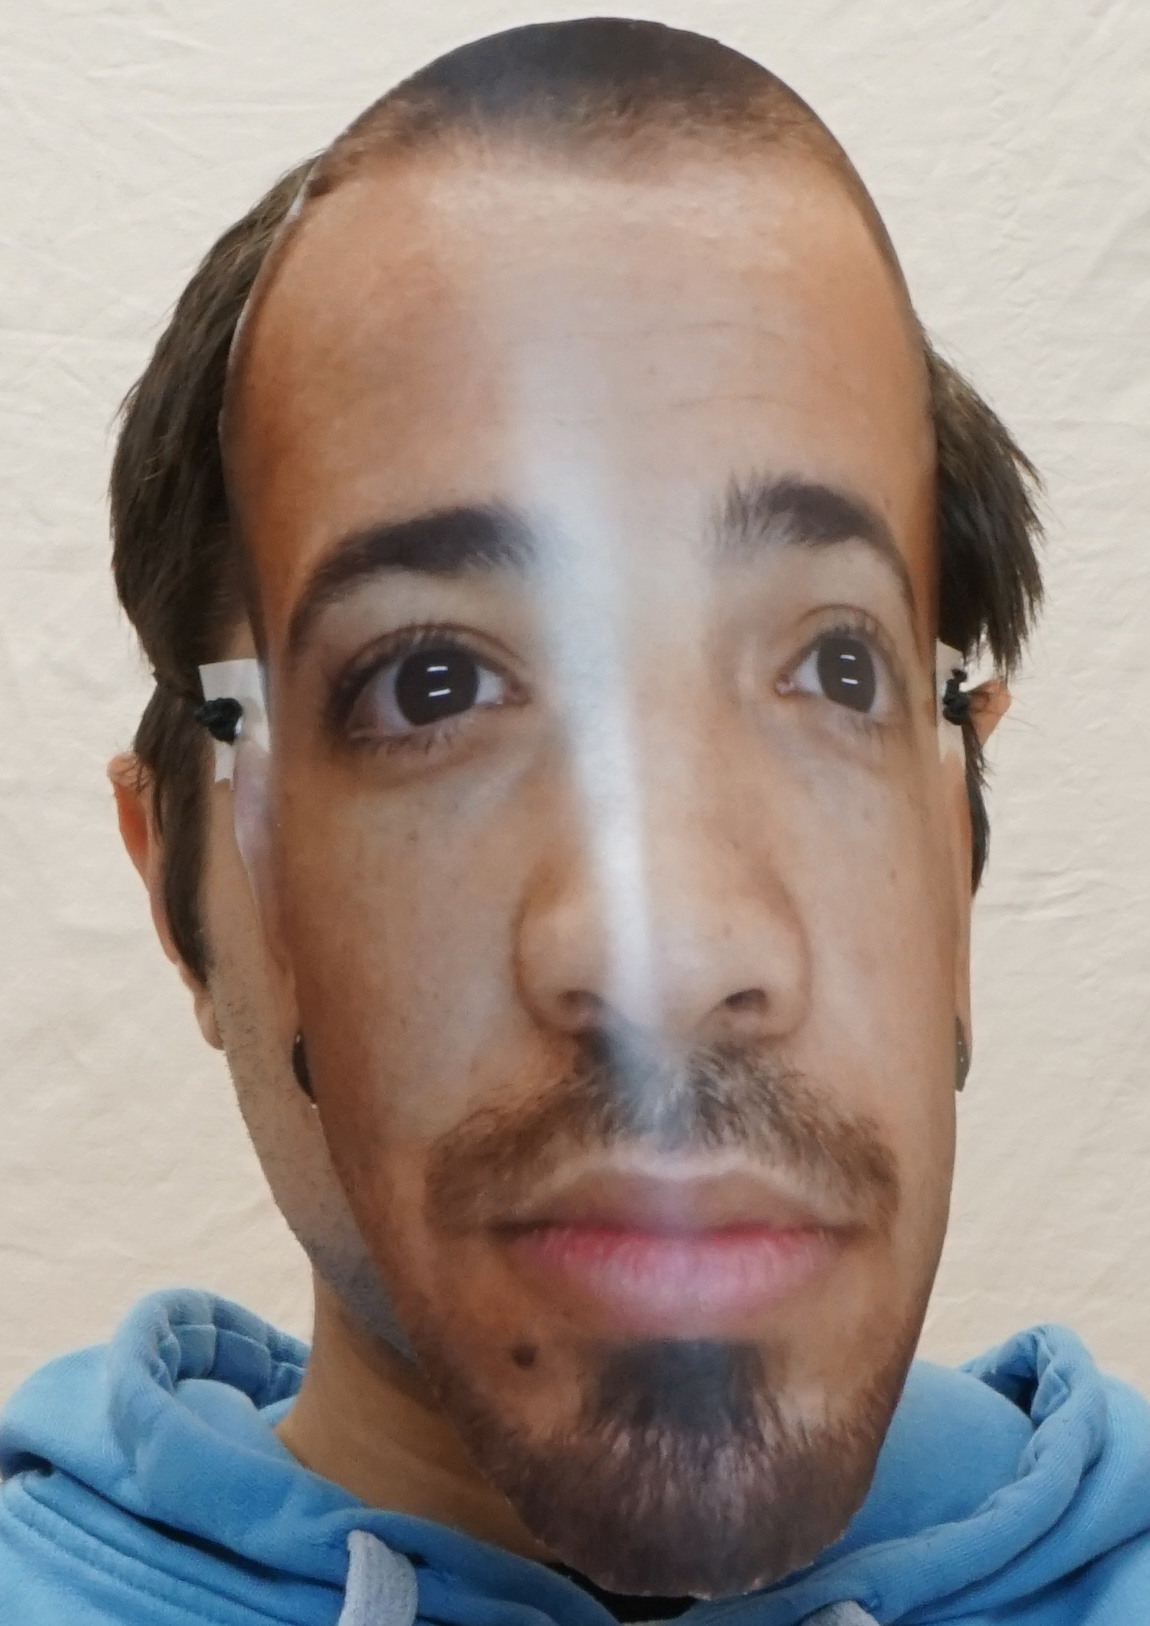
\includegraphics[width=0.18\textwidth]{images_databases/fravrgb/at2-1.JPG} \label{frav_im2-2}}
\subfigure[eye mask attack RGB]{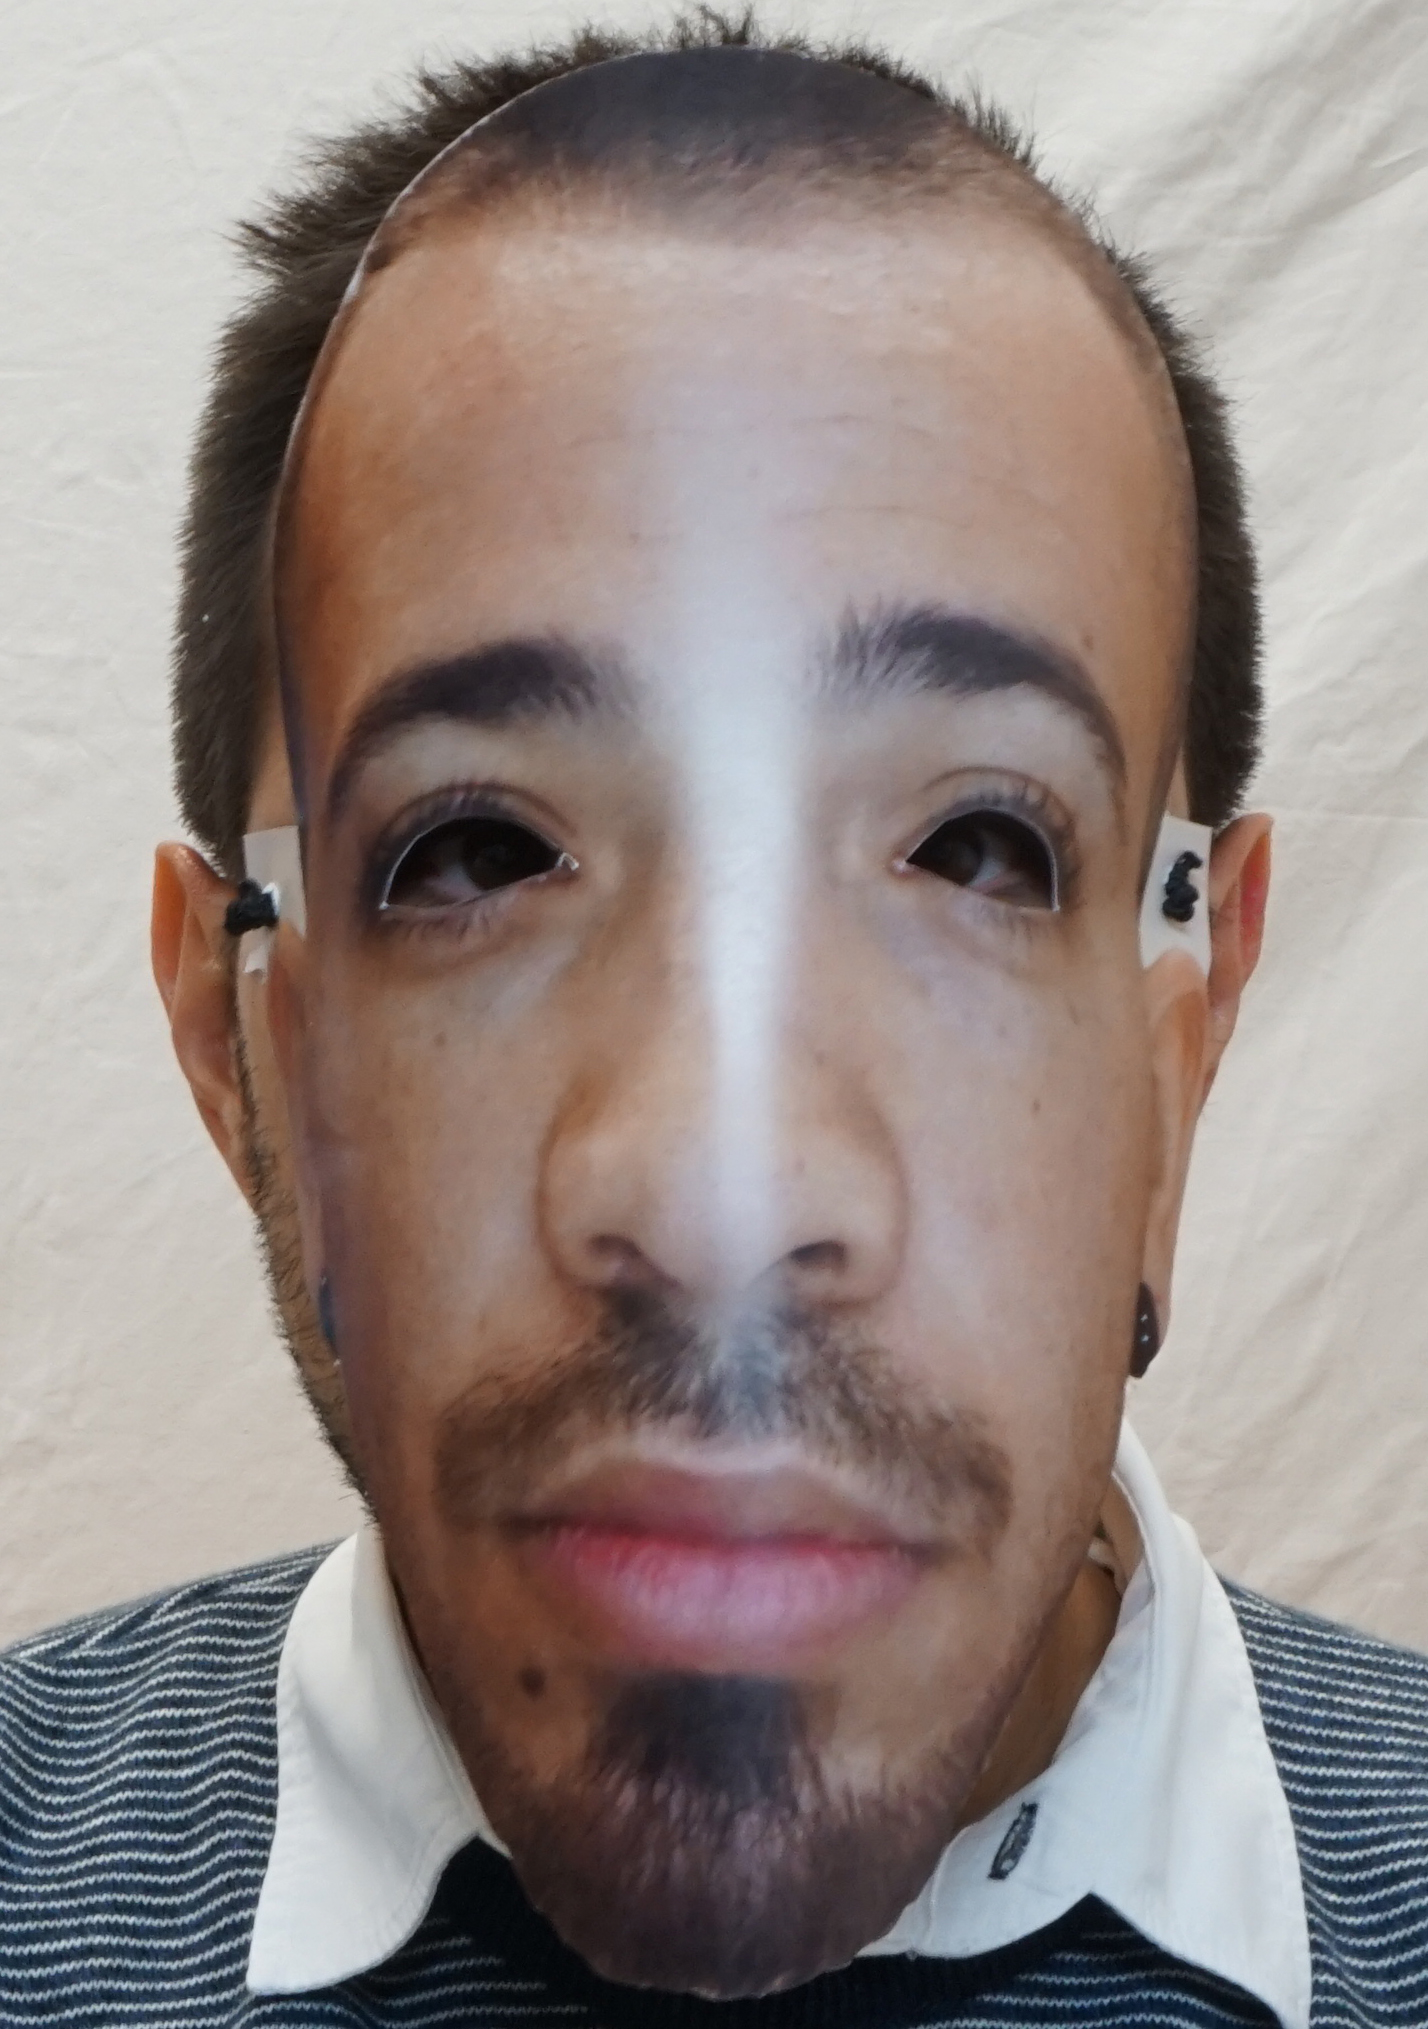
\includegraphics[width=0.18\textwidth]{images_databases/fravrgb/at3-1.JPG} \label{frav_im2-3}}
\subfigure[tablet attack RGB]{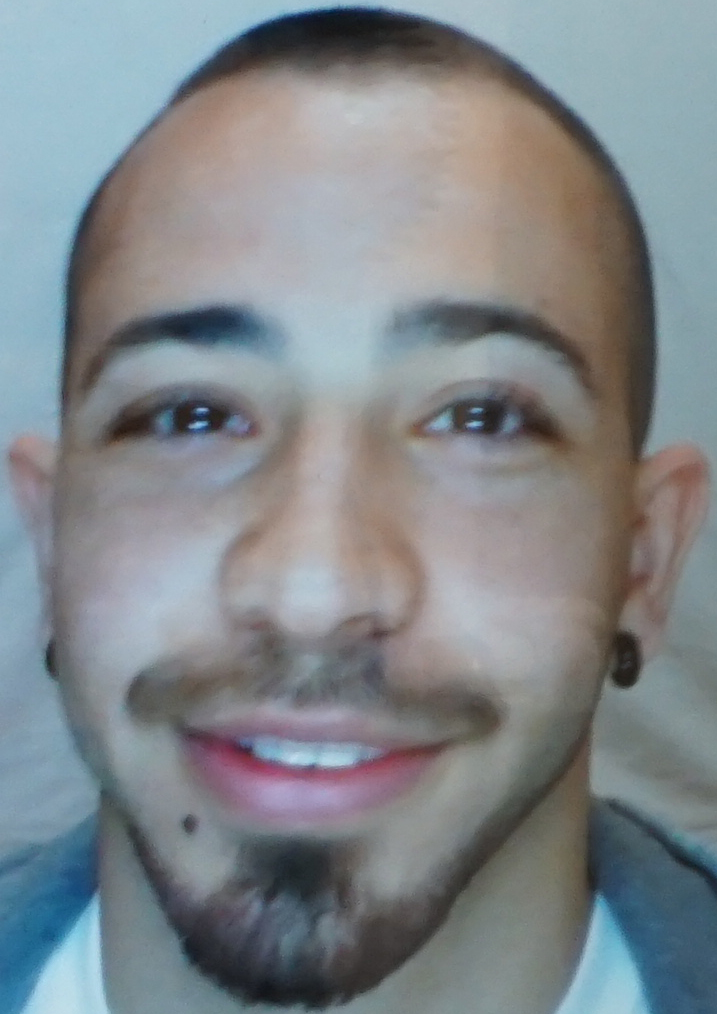
\includegraphics[width=0.18\textwidth]{images_databases/fravrgb/at4-1.JPG} \label{frav_im2-4}}
\subfigure[real user RGB]{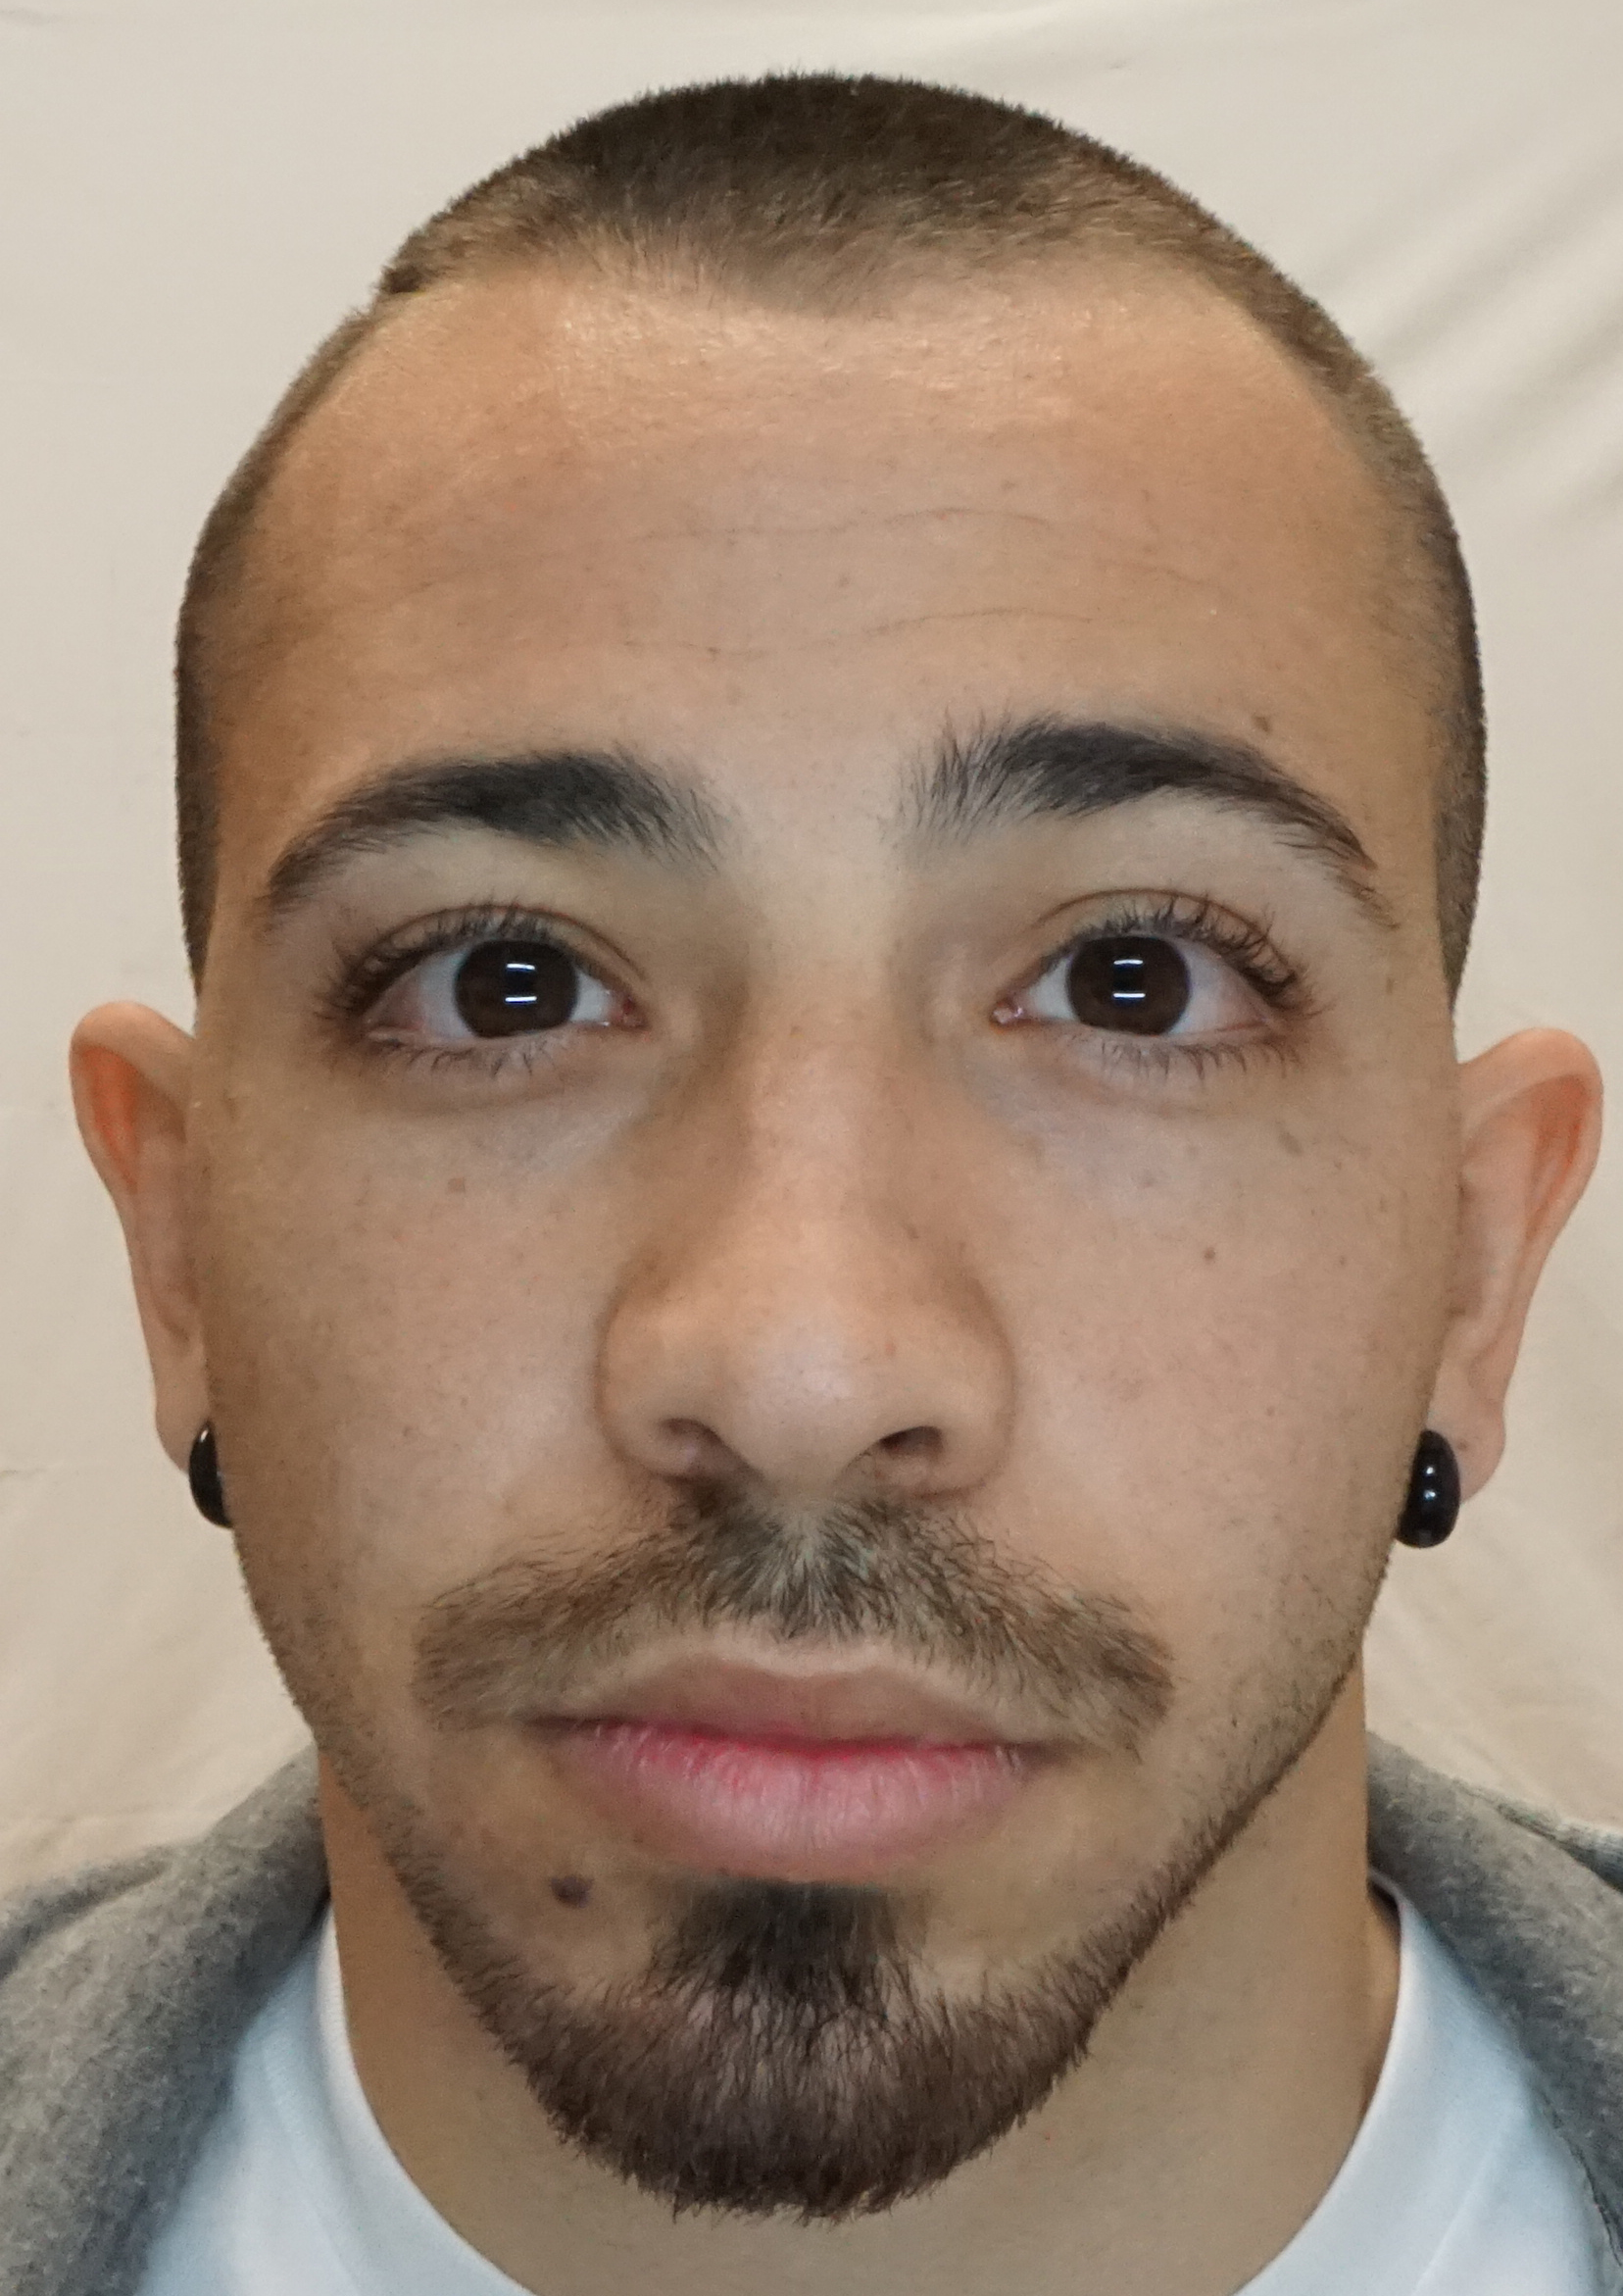
\includegraphics[width=0.18\textwidth]{images_databases/fravrgb/real1.JPG} \label{frav_im2-5}}

\subfigure[printed NIR image attack]{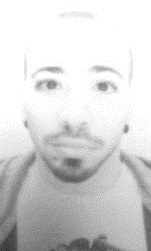
\includegraphics[width=0.18\textwidth]{images_databases/fravnnir/at-1.jpg} \label{frav_im3-1} }
\subfigure[mask attack NIR]{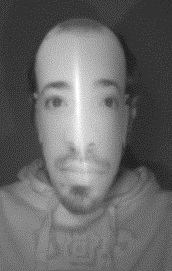
\includegraphics[width=0.18\textwidth]{images_databases/fravnnir/at-2.jpg} \label{frav_im3-2}}
\subfigure[eye mask attack NIR]{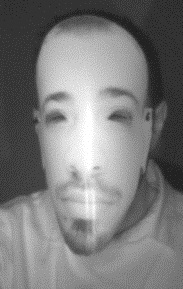
\includegraphics[width=0.18\textwidth]{images_databases/fravnnir/at-3.jpg} \label{frav_im3-3}}
\subfigure[tablet attack NIR]{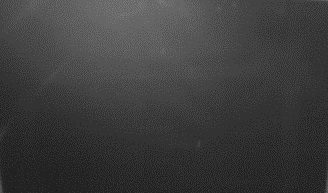
\includegraphics[width=0.18\textwidth]{images_databases/fravnnir/at-4.jpg} \label{frav_im3-4}}
\subfigure[real user NIR]{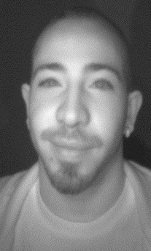
\includegraphics[width=0.18\textwidth]{images_databases/fravnnir/real.jpg} \label{frav_im3-5}}

\caption{Four attacks and real user of RGB and NIR FRAV database } \label{fig:RGB-frav2}
\end{figure}

As could be seen in figure \ref{fig:RGB-frav1} and figure \ref{fig:RGB-frav2}, five different classes composes this database. One class is the real user class and the other four classes are four spoofing attacks per user:

\begin{itemize}
 \item Original images of people represented in figure \ref{frav_im1-4} and figure \ref{frav_im2-5} for RBG images and figure \ref{frav_im3-5} for NIR image.
 \item Images of people printed (attack) represented in figure \ref{frav_im1-1} and figure \ref{frav_im2-1} for RBG images and figure \ref{frav_im3-1} for NIR image.
 \item Images of people with a mask (attack)represented in figure \ref{frav_im1-2}and figure \ref{frav_im2-2}for RBG images and figure \ref{frav_im3-2} for NIR image.
 \item Images of people with a mask with the eyes cropped (attack)represented in figure \ref{frav_im1-3} and figure \ref{frav_im2-3} for RBG images and figure \ref{frav_im3-3} for NIR image.
 \item Images of people in a tablet (attack)represented in figure \ref{frav_im1-4} and figure \ref{frav_im2-4} for RBG images and figure \ref{frav_im3-4} for NIR image.\\
 \end{itemize}

Images of classes can be found in RGB and NIR (not all RGB images has its corresponding NIR image). Characteristics of FRAV images database are the following ones:

\begin{itemize}[noitemsep,topsep=8pt,parsep=0pt,partopsep=20pt]
\item There are 939 people in each RGB class or 195 in each NIR class.
\item There is one image per person.
\item Each image has it is own shape.
\item As it real user has all the four attack, all the classes has the same number of samples.
\item The faces are centered in the image.
\end{itemize}

This database is used in two different ways:

\begin{enumerate}
  \item Using only RGB images (figure \ref{fig:RGB-frav1}), where there are 933 people, in which each person would have a genuine image and four attack, so 4665 samples are available.
  \item Using the RGB and NIR images, where there are 195 people which correspond with NIR images and its corresponding images in RGB. 975 samples are available.
\end{enumerate}

If RGB and NIR (figure \ref{fig:RGB-frav2})images are used at the same time, two different methods, for using both types of images together, are used:
\begin{itemize}
\item Characteristic level: adding the NIR image as another layer to RGB image, so the resultant image have hightxweightx4 dimensions (NIR images has one layer because it is a gray scale image and RGB images has tree layers, one per each primary color). The network is feed with the resultant images like other times.
\item Classification level: after the network training and before feeding the classifier, RGB and NIR would be trained separately and its features would be appended as the input of the classifier.
\end{itemize}

To conclude, this database is going to be used in the three different ways: just RGB images, RGB and NIR images added in characteristic level or classification level.\\

When the classes are build, two ways are possible to be done: the first one where real people are one class (positive) and the different attacks are other class (negatives), so two classes have been used; and the second way where each attacks correspond with a class, so five classes (4 attacks and 1 real) have been used.\\


\subsection{CASIA dataset}
The CASIA Face Anti-Spoofing database is a database from the Chinese Academy of Sciences Centre for Biometrics and Security Research (CASIA-CBSR) \cite{Casiadatbase}.

A person of CASIA database could be seen in figure \ref{fig:casia2}, where three attacks types could be seen (figure \ref{casia_im1-1}, \ref{casia_im2-1} and \ref{casia_im3-1} ) with the real user (figure \ref{casia_im4-1}). \\

\begin{figure}[htb]
\centering
\subfigure[printed image attack]{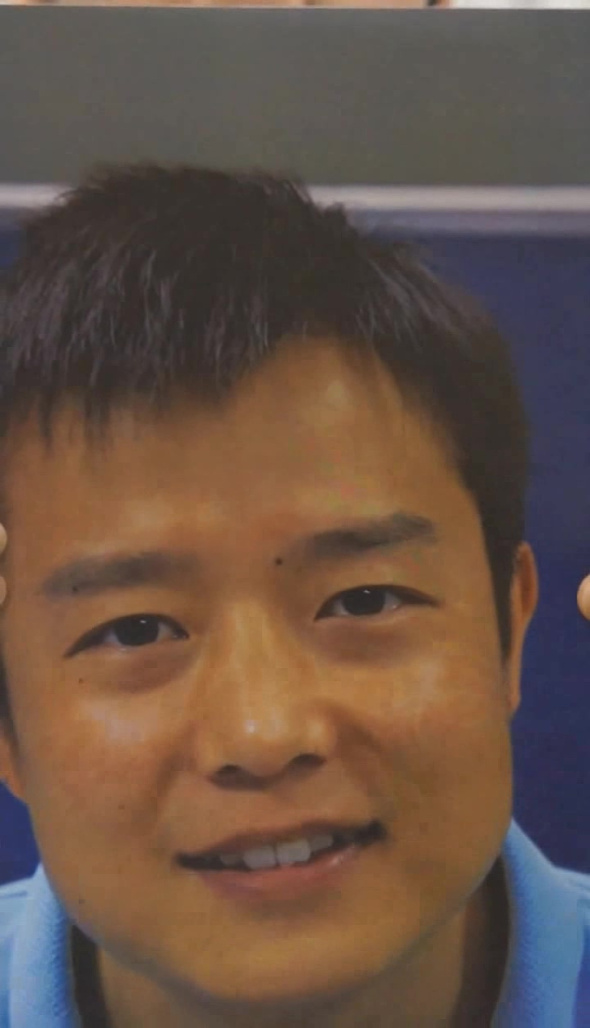
\includegraphics[width=0.2\textwidth]{images_databases/casia/at1-2.jpg} \label{casia_im1-1} }
\subfigure[eye printed image attack]{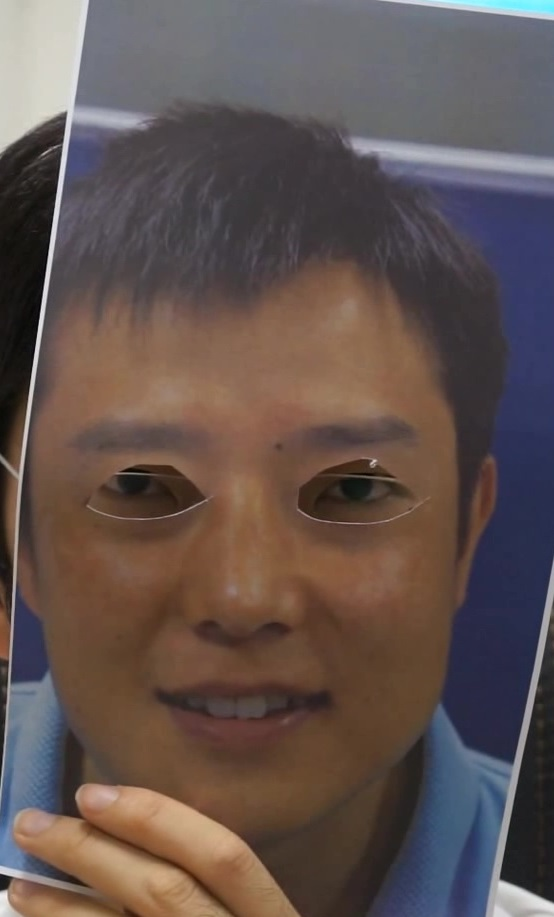
\includegraphics[width=0.2\textwidth]{images_databases/casia/at2-2.jpg} \label{casia_im2-1} }
\subfigure[tablet attack]{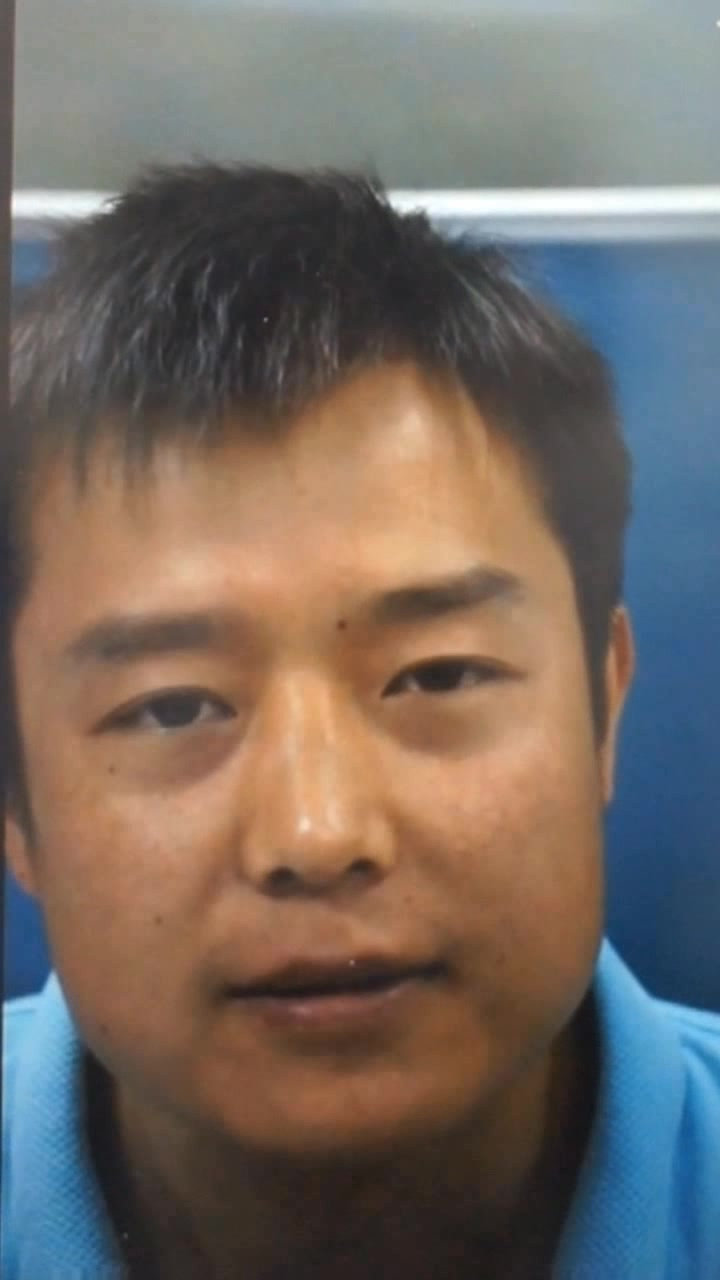
\includegraphics[width=0.2\textwidth]{images_databases/casia/at3-2.jpg} \label{casia_im3-1} }
\subfigure[real user]{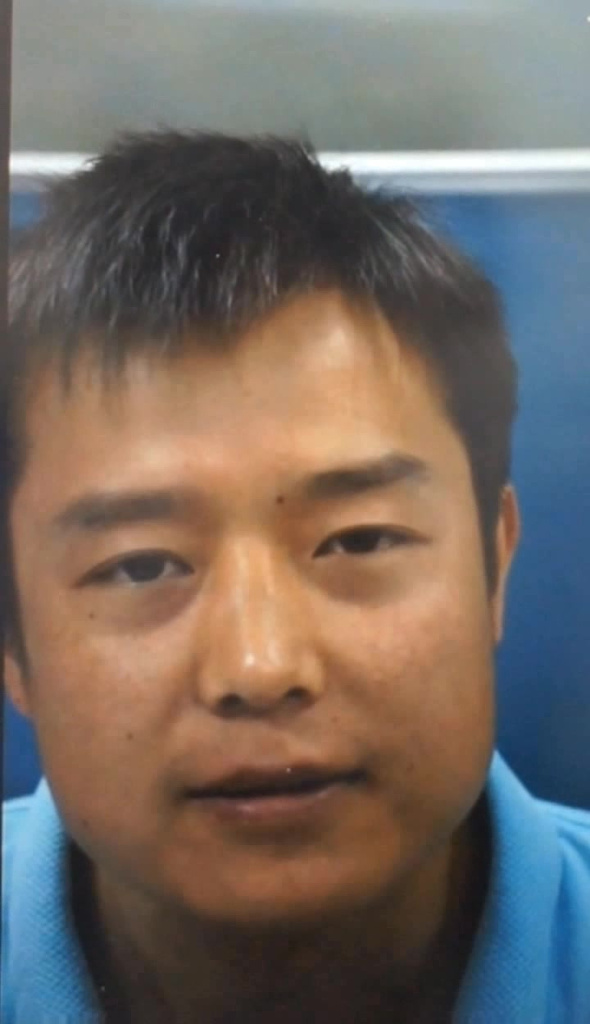
\includegraphics[width=0.2\textwidth]{images_databases/casia/real2.jpg} \label{casia_im4-1} }

\caption{Three attacks and real user from casia database } \label{fig:casia2}
\end{figure}

In the same way as FRAV dataset, this database is formed by real or genuine images of people and three different attacks of the same people:
\begin{itemize}[noitemsep,topsep=8pt,parsep=0pt,partopsep=20pt]
 \item Images of people printed (attack) represented in figure \ref{casia_im1-1}.
 \item Images of people with a mask with the eyes cropped (attack) represented in figure \ref{casia_im2-1}.
 \item Tablet attack represented in figure \ref{casia_im3-1}
  \item Images of real users represented in figure \ref{casia_im4-1}.
 \end{itemize}

Originally, this database is a video database, in which each sample is a different video, but for the experiments developed no videos (entirely or fed directly to the network) have been used. The CASIA database has been used in two different ways:
\begin{itemize}
 \item Using a single image per person and class. When this database is used, it is going to be referred as CASIA image database.
 \item Reading three frames per video and saving each frame as a independent image sample. This database is going to be referred as CASIA video database.
\end{itemize}

The characteristics of the CASIA image database are the following ones:
\begin{itemize}[noitemsep,topsep=8pt,parsep=0pt,partopsep=20pt]
\item There are 49 images per user, so there are 196 unique samples.
\item Samples do not have the same size.
\item Samples are in RGB space.
\item The face of the image is centered.
\end{itemize}

The characteristics of the CASIA video database are the following ones:
\begin{itemize}
\item There are 8 videos per person (two videos for real user, and two per each attack). There are two videos because one is filmed horizontally and the other vertically, one filmed with a smartphone and the other with the frontal camera of a laptop.
\item There are 50 different users, so there are 400 different videos.
\item For each video 3 frames are read, so there are 1200 unique samples.
\item Samples are in RGB space.
\item Faces are centered in the image and blink expression and movement of people are produced.
\end{itemize}

At the time of assigning a class, it could be done using two classes, the positive class to the real users and the negative class to the attacks; If each attack is assigned to a independent class, it would be four different classes, the real user class and three attack classes.\\

%\begin{figure}[htb]
%\centering
%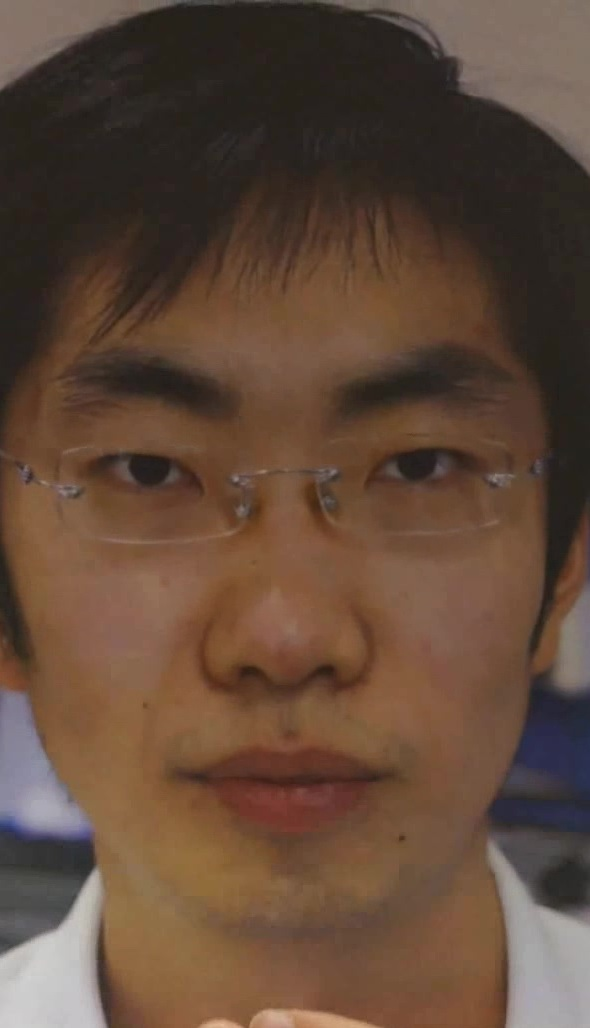
\includegraphics[width=0.2\textwidth]{images_databases/casia/at1-1.jpg}
%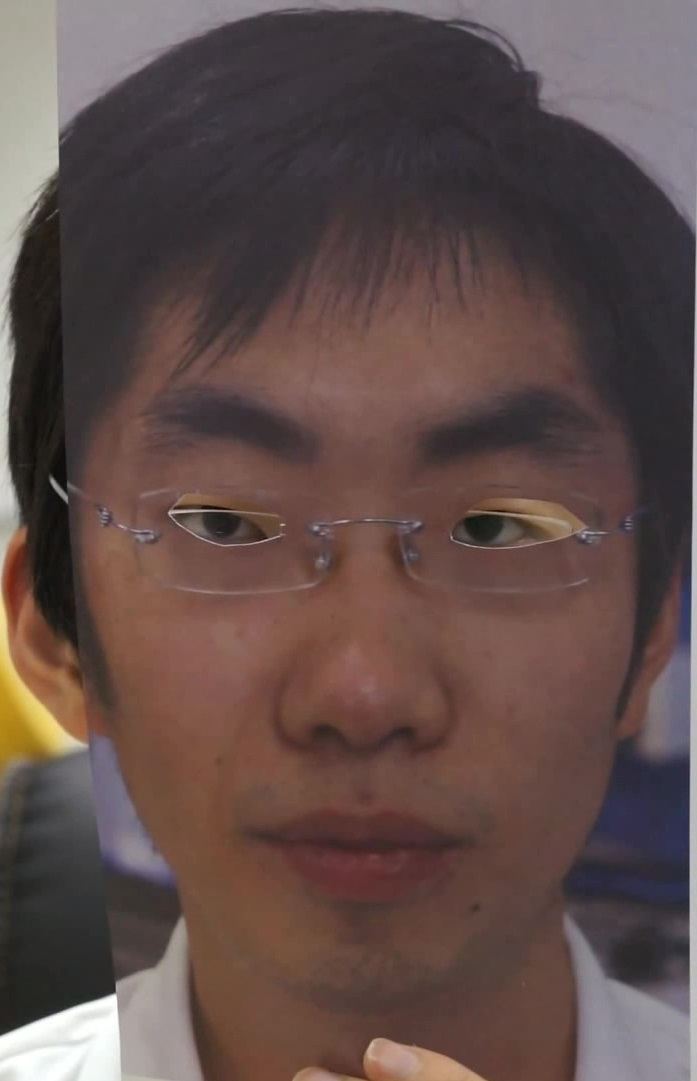
\includegraphics[width=0.2\textwidth]{images_databases/casia/at2-1.jpg}
%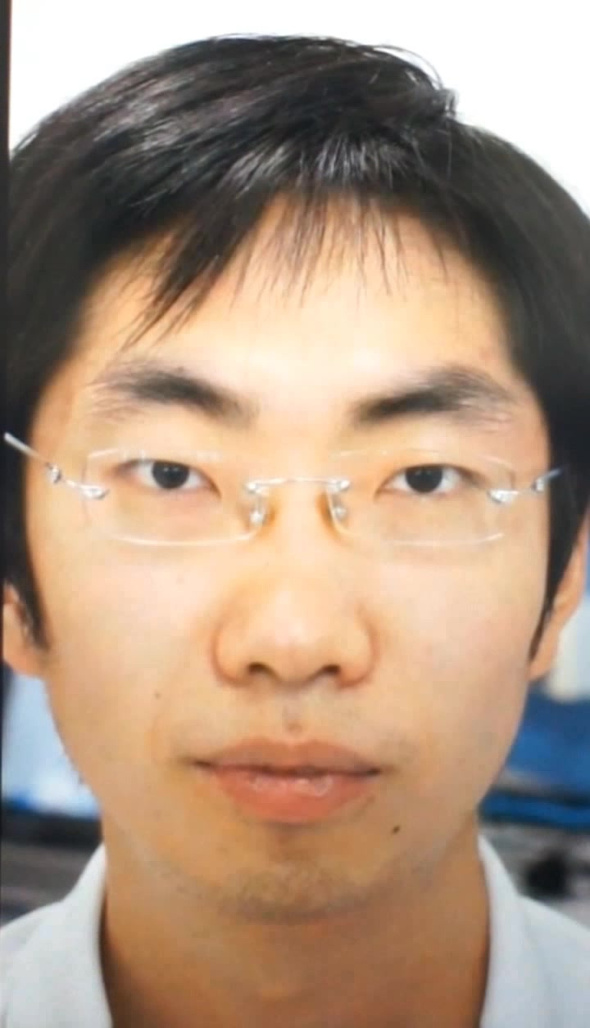
\includegraphics[width=0.2\textwidth]{images_databases/casia/at3-1.jpg}
%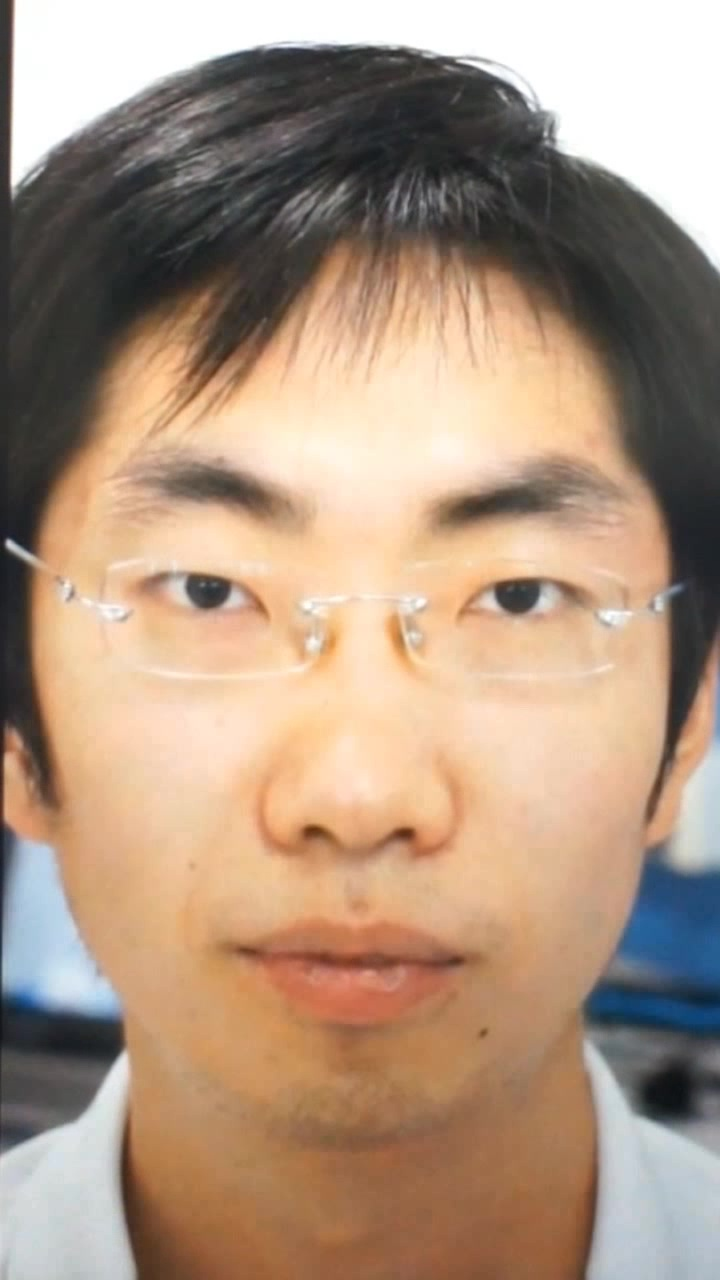
\includegraphics[width=0.2\textwidth]{images_databases/casia/real1.jpg}

%\caption{Three attacks and real user from casia database } \label{fig:casia1}
%\end{figure}

This database has been used in different articles \cite{yangLL14,Spoofing_survey,MSUdatabse,LSTM-CNN} it is a very used databased for face biometrics.\\

\subsection{MSU - MFSD database}
The MSU Mobile Face Spoofing Database (MFSD) is a video face anti-spoofing database \cite{MSUdatabse}.\\

In figure \ref{fig:mfsd} are represented the three attacks and a real user which forms this database:
\begin{itemize}[noitemsep,topsep=8pt,parsep=0pt,partopsep=20pt]
\item Printed photo attack represented in figure \ref{mfsd_im1-1}.
\item Tablet attack where a video is Replayed represented in figure \ref{mfsd_im1-1}.
\item Smartphone attack represented in figure \ref{mfsd_im1-1}.
\item Real user represented in figure \ref{mfsd_im1-1}.
\end{itemize}

\begin{figure}[htb]
\centering
\subfigure[printed image attack]{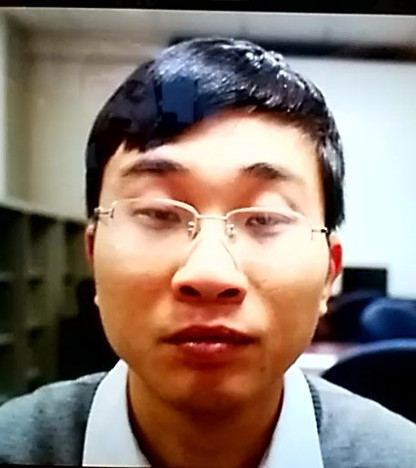
\includegraphics[width=0.2\textwidth]{images_databases/MFSD/at1-1.jpg} \label{mfsd_im1-1} }
\subfigure[tablet attack]{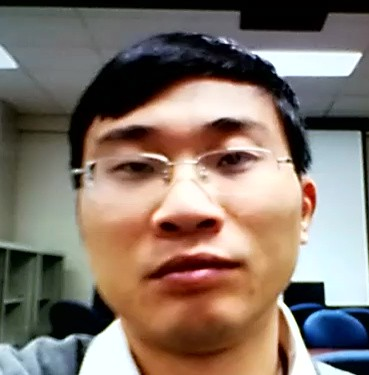
\includegraphics[width=0.2\textwidth]{images_databases/MFSD/at2-1.jpg} \label{mfsd_im2-1} }
\subfigure[smartphone attack]{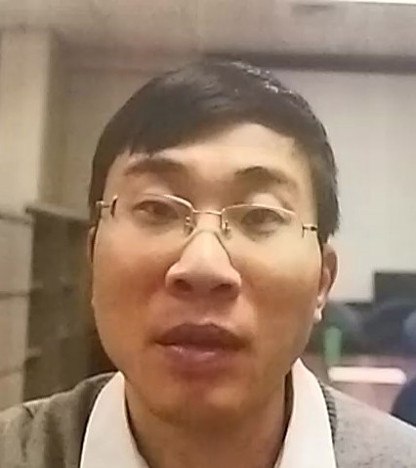
\includegraphics[width=0.2\textwidth]{images_databases/MFSD/at3-1.jpg} \label{mfsd_im3-1} }
\subfigure[real user]{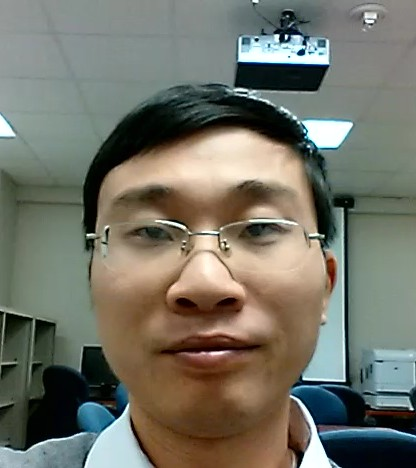
\includegraphics[width=0.2\textwidth]{images_databases/MFSD/1.jpg} \label{mfsd_im4-1} }

\caption{Three attacks and  real user from a person of MFSD database } \label{fig:mfsd}
\end{figure}

Originally, the database is a video one, but just one image per user and class is used. The characteristics of the database are the following ones:
\begin{itemize}[noitemsep,topsep=8pt,parsep=0pt,partopsep=20pt]
\item There are 35 images per attack or genuine user. There are 140 unique samples.
\item Images are in RGB space.
\item Faces are centred in images.
\item The size of each image are not equal. Approximately images are 300 pixel heigh and 335 pixel width.
\end{itemize}

%\begin{figure}[htb]
%\centering
%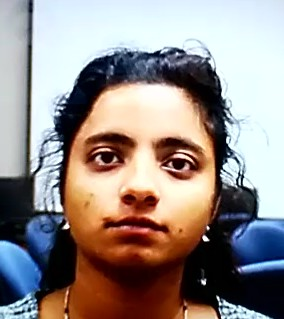
\includegraphics[width=0.2\textwidth]{images_databases/MFSD/at1-2.jpg}
%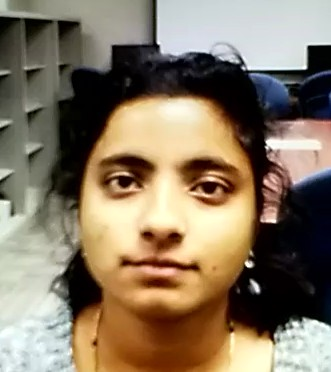
\includegraphics[width=0.2\textwidth]{images_databases/MFSD/at2-2.jpg}
%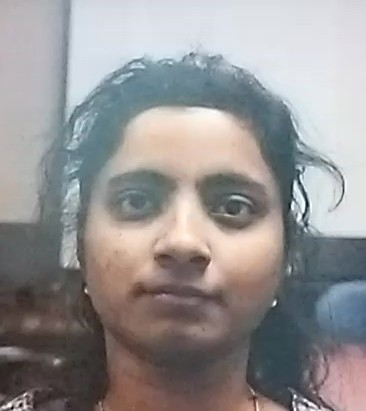
\includegraphics[width=0.2\textwidth]{images_databases/MFSD/at3-2.jpg}
%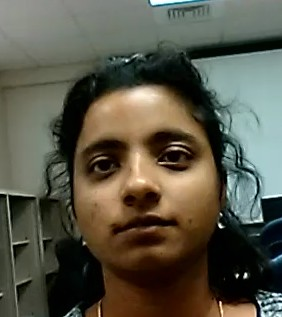
\includegraphics[width=0.2\textwidth]{images_databases/MFSD/2.jpg}
%\caption{Three attacks and real user from a user of MFSD database } \label{fig:mfsd2}
%\end{figure}
